\begin{figure*}
\begin{center}

\begin{minipage}{\linewidth}
\begin{subfigure}[b]{\linewidth}
\begin{minipage}{0.5\textwidth}
\begin{center}
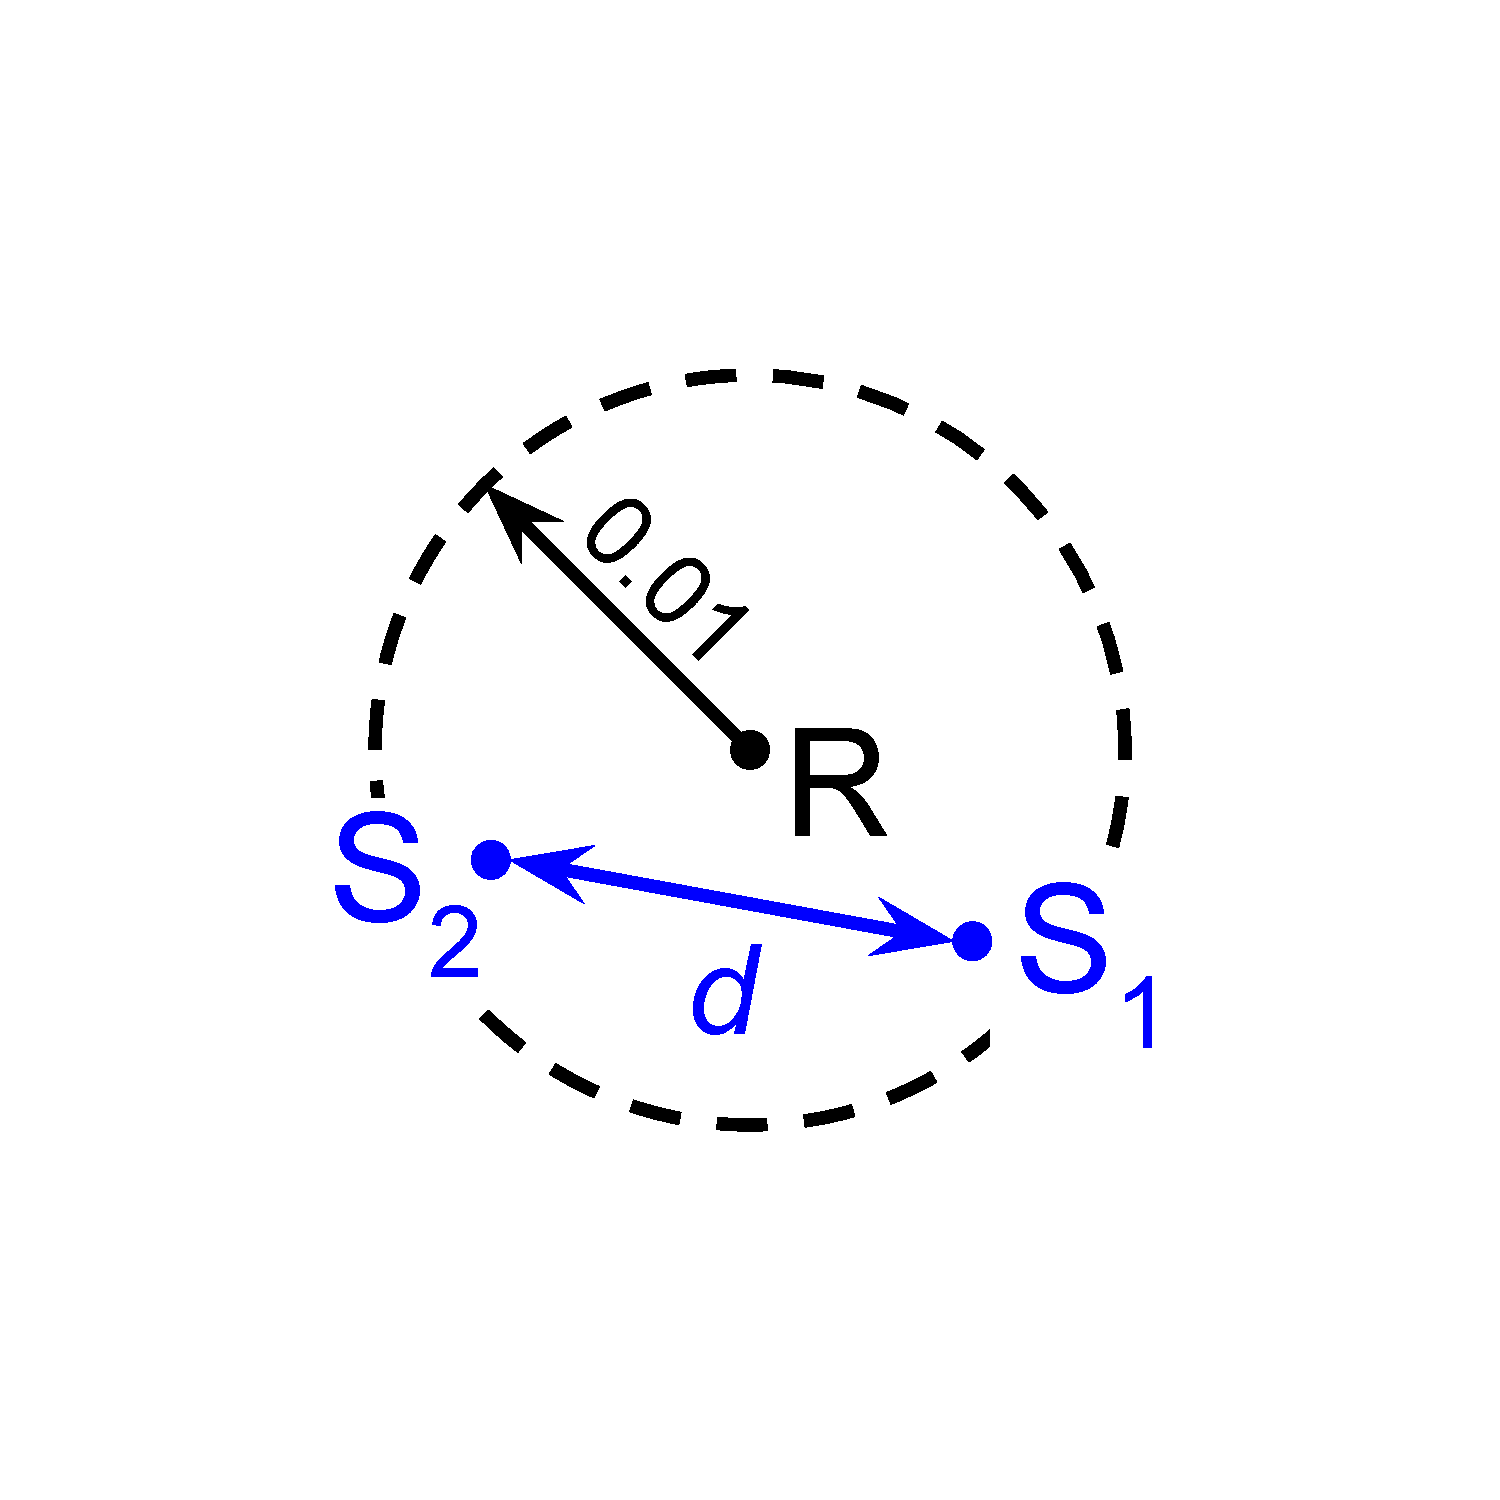
\includegraphics[width=0.5\linewidth,trim=5cm 5cm 5cm 5cm, clip]{img/dimensionality-statistic}
\end{center}
\end{minipage}%
\begin{minipage}{0.5\textwidth}
\caption{
Sampling process used to measure similarity constraint.
First, a constraining tag $R$ was randomly sampled.
Then, tags were randomly drawn until two tags $S_1$ and $S_2$ with distance to $R$ less than 0.01 were obtained.
Finally, similarity constraint was measured as the distance $d$ between $S_1$ and $S_2$.
}
\label{fig:dimensionality_measure}
\end{minipage}
\end{subfigure}
\end{minipage}
\begin{subfigure}[b]{\linewidth}
\begin{minipage}{0.6\linewidth}
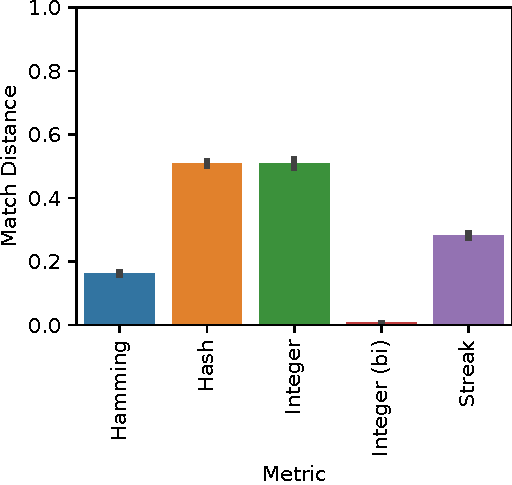
\includegraphics[width=\linewidth]{img/sphere/bitweight=0dot5+seed=1+title=dimensionality_barplot+_data_hathash_hash=c0f6c5cf854ff253+_script_fullcat_hash=03ce1e318a24a109+ext=}
\end{minipage}
\begin{minipage}{0.35\linewidth}
\caption{
Mean similarity constraint.
Error bars represent 95\% confidence intervals.
}
\label{fig:sphere_barplot}
\end{minipage}
\end{subfigure}
\begin{minipage}{\linewidth}
\begin{subfigure}[b]{\linewidth}
\centering
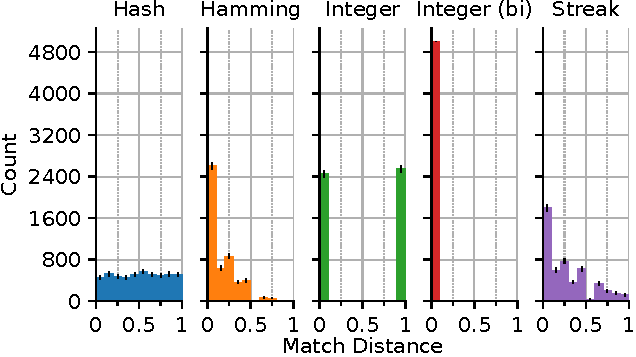
\includegraphics[width=\linewidth]{img/sphere/bitweight=0dot5+seed=1+title=dimensionality_distnplot+viz=hist+_data_hathash_hash=c0f6c5cf854ff253+_script_fullcat_hash=290cd520ead87cd0+ext=}
\begin{minipage}{0.8\textwidth}
\caption{
Frequency of sampled similarity constraint values in each match distance decile.
Error bars are 95\% confidence intervals calculated using the Wilson score method with continuity correction \citep{newcombe1998two}.
}
\label{fig:sphere_distnplot}
\end{minipage}
\end{subfigure}
\end{minipage}

\caption{
Similarity constraint of tag-matching metrics.
Figure \ref{fig:dimensionality_measure} summarizes the sampling process used to measure similarity constraint.
Figures \ref{fig:sphere_barplot} and \ref{fig:sphere_distnplot} compare distributions of similarity constraint across metrics.
}
\label{fig:sphere}

\end{center}
\end{figure*}
